% Emacs, this is -*-latex-*-

\title{Information Theory}
\maketitle

\tableofcontents

\section{Rate}

In a communication system, the
\href{https://en.wikipedia.org/wiki/Bit_rate}{rate} describes the
amount of data (for example, bits) that is transmited by time unit
(for example, a second).

\section{Distortion}

In an lossy encoding system, the distortion (expressed for example by
the \href{https://en.wikipedia.org/wiki/Mean_squared_error}{MSE})
measures the amount of error between two signals: the original signal
and the distorted one. The origin of this error can be quite varied
and ranges from transmission errors to quantization processes.

\section{RD (Rate/Distortion) curve}

\begin{figure}
  \centering
  %\svgfig{graphics/RD_slopes}{8cm}{800}
  %\svg{graphics/RD_slopes}{800}
  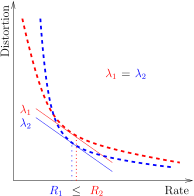
\includegraphics[width=1.0\textwidth]{graphics/RD_slopes} 
  \caption{Two RD (Rate/Distortion) curves.}
  \label{fig:RD_slopes}
\end{figure}

For example, when the signal is quantized, rate and distortion are
``conflicting'' features of the encoding system in the sense that, for
example, if the bit-rate is descreased, the distortion is increased,
and viceversa. Such variables (Rate (R) and Distortion (D)) can be
represented as a curve such as the shown in the
Fig.~\ref{fig:RD_slopes}. Usually, RD curves are convex, which means
that if $\lambda_i$ is the slope of the curve measured at the $i$-th
point of the curve (starting at the lowest bit-rate), it usually hold
that
\begin{equation}
  \lambda_i > \lambda_{i+1}.
  \label{eq:convexity}
\end{equation}
where $\lambda$ quantifies the trade-off between decreasing the
distortion\footnote{For this reason, the slopes are negative.} while
the bit-rate
increases~\cite{vetterli1995wavelets,sayood2017introduction}. However,
Eq.~\eqref{eq:convexity} is not always true in the real world.

%}}}

\section{Resources}
%{{{ 
\renewcommand{\addcontentsline}[3]{}% Remove functionality of \addcontentsline
\bibliography{data-compression,signal-processing,DWT}
%}}}
